\section{Motivation}

% The idea for this work comes from a recent paper that proposed a technique based on a neural formulation of EVPI in the context of forum posts, e.g., Stack Exchange, intending to augment such posts with edits that improve their quality~\cite{rao-daume-iii-2018-learning}. Our work focuses on bug reports and uses a different formulation of EVPI that is better suited to both the diversity of bug reports and to the specific ways bug reports can be improved via follow up questions.


Motivation of the problem:

The problem is real, i.e., there are repos that have more BRs than they can manage. How many BRs arrive at the most popular repos (is the traffic bursty)? how many lack OB/EB/S2R from these?

\begin{figure*}[t]
\centering
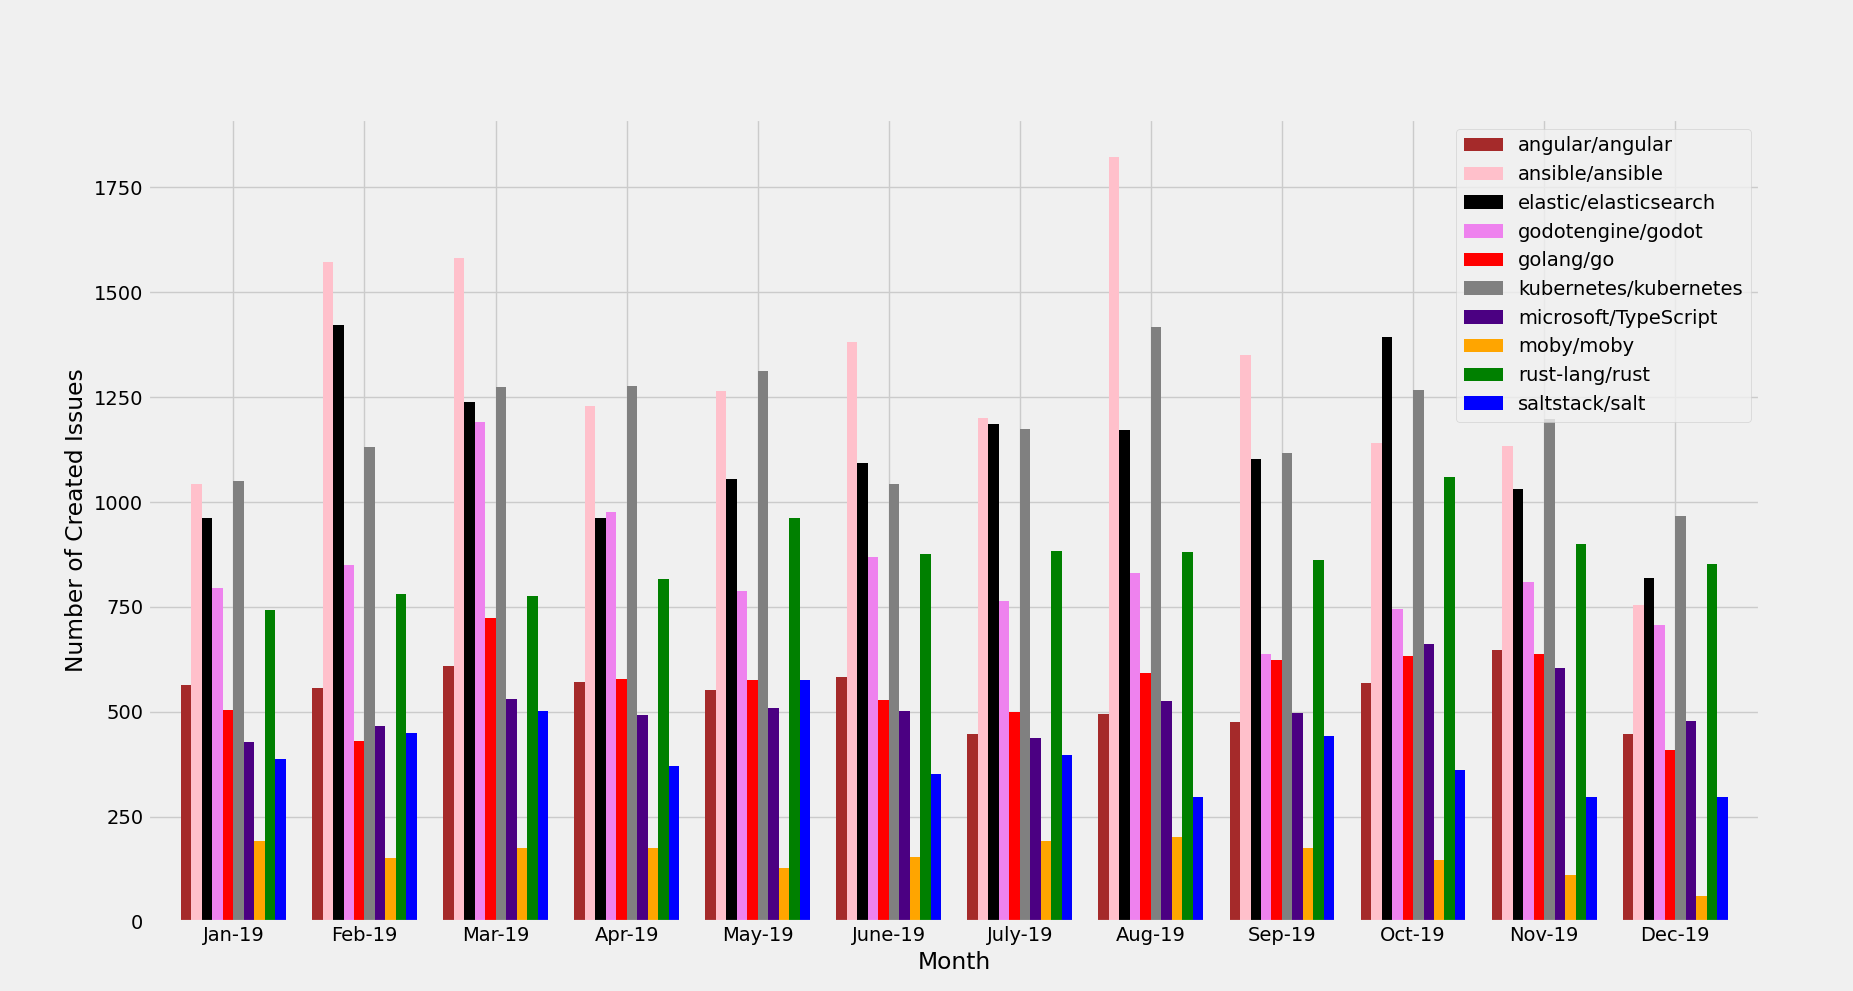
\includegraphics[width=0.79\linewidth]{figures/repos_month_bar.png}
\caption{...}
\label{fig:repo_activity}
\end{figure*}



The preconditions are present, i.e., there are a lot of follow-up questions on GitHub






Motivate the value of the answer as a way of ranking
